\subsection{地理知识}

\begin{quote}
	本部分主要参考人教版普通高中教科书《地理》必修和选修教材,结合部分行测真题考点写成。
\end{quote}

\subsubsection{地球的大气}

\paragraph{大气组成}

低层大气中除去水汽和杂质以外的混合气体,称为干洁空气。25千米以下的干洁空气主要由氮气(78\%)、氧气(21\%)、二氧化碳(0.03\%)和氩气等组成。大气中氧气含量对人体健康至关重要。科学研究发现,\textbf{适当的缺氧环境利于激发运动员的运动潜力。}但含氧量太低会危害人体健康甚至危及生命。

\paragraph{大气分层}

大气主要分为对流层,平流层,高层大气。对流层集中了大气圈质量的 3/4和几乎全部的水汽、杂质,大气中的污染物也多集中在这一层。对流层的高度因纬度而异,在低纬度地区为 17—18千米,在高纬度地区仅为 8—9千米。对流层气温随高度的升高而递减,在对流层的顶部气温降至 –60℃。平流层范围自对流层顶部至 50—55 千米高空。平流层气温随高度升高而升高。该层大气的下层气温随高度变化很小,但是在 30 千米以上,气温随高度增加而迅速上升。这是因为平流层中的臭氧吸收大量太阳紫外线,使大气增温。在 22—27 千米范围内,臭氧含量达到最大值,形成臭氧层。臭氧层使地球上的生命免受过多紫外线的伤害,被称为“地球生命的保护伞”。平流层以上的大气统称高层大气。自平流层顶部开始,由于没有吸收紫外线的臭氧,气温会下降;随后,由于大气吸收了更短波长的太阳紫外线,温度又持续上升,在 300 千米的高空,温度可达 1 000℃以上。

\paragraph{大气的受热}

大气受热主要依靠地面长波辐射。太阳的短波辐射只占小部分。同时大气也向地面辐射大部分长波辐射,称作大气逆辐射,对地面起到保温作用。

\begin{figure}[h]
	\centering
	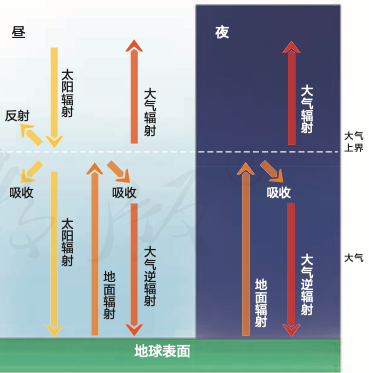
\includegraphics[width=0.8\textwidth]{assets/images/地理知识-01.png}
	\caption{大气受热示意图}
	\label{fig:大气受热}
\end{figure}

\paragraph{大气热力环流}

大气热力环流是一种常见的自然现象。在一定条件下,地表的冷、热差异会产生大气热力环流。台湾海峡两岸风向的日变化,反映了海陆间大气热力环流的日变化,城市热岛效应也是大气热力环流的一种表现。

\paragraph{大气的水平运动——风}

空气受到水平气压梯度力,地转偏向力和摩擦力作用,形成风。

\begin{figure}[h]
	\centering
	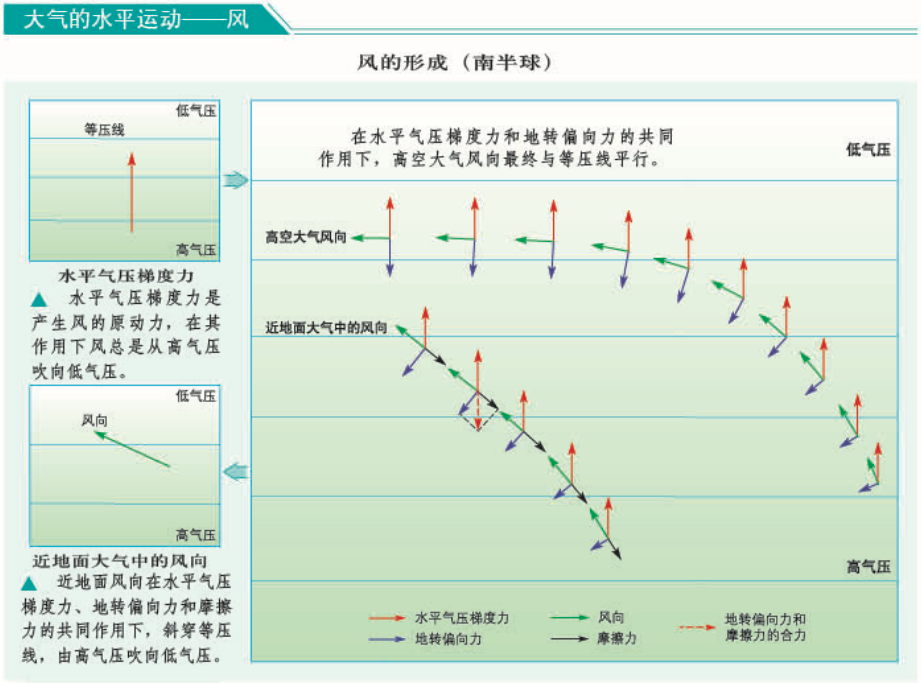
\includegraphics[width=0.8\textwidth]{assets/images/地理知识-02.png}
	\caption{风的形成示意图}
	\label{fig:风的形成}
\end{figure}
